% usv_frame.tex
% Standalone LaTeX figure: USV coordinate frames (inertial + body + horizontal projection)
% Compile: pdflatex usv_frame.tex
\documentclass[tikz,border=6pt]{standalone}

\usepackage{ctex} % for Chinese labels; remove if you prefer English-only
\usepackage{tikz}
\usetikzlibrary{arrows.meta,calc}


\begin{document}
\begin{tikzpicture}[>=Stealth, line cap=round, line join=round]

% ---------- Inertial frame ----------
\begin{scope}
  \node at (-3.0,1.6) {惯性坐标系};

  \draw[thick,->] (-4,0) -- (-2.8,0) node[above] {$x_0$};
  \draw[thick,->] (-4,0) -- (-4,-1.2) node[right] {$z_0$};
  \draw[thick,->] (-4,0) -- (-5.2,0.8) node[left] {$y_0$};

  \node[below left] at (-4,0) {$o_0$};
\end{scope}

% ---------- USV body frame ----------
\begin{scope}[xshift=2.2cm]

  % USV outline (simplified)
  \draw[thick] (-1.2,0.2) .. controls (0,0.6) .. (1.4,0.2);
  \draw[thick] (-1.2,-0.2) .. controls (0,-0.6) .. (1.4,-0.2);
  \draw[thick] (-1.2,0.2) -- (-1.2,-0.2);
  \draw[thick] (1.4,0.2) -- (1.4,-0.2);

  \node at (0,1.2) {附体坐标系};

  % Body axes
  \draw[thick,->] (0,0) -- (1.6,0) node[above] {$x$};
  \draw[thick,->] (0,0) -- (0,-1.2) node[right] {$z$};
  \draw[thick,->] (0,0) -- (-0.9,0.6) node[left] {$y$};

  \node[left] at (0,0) {$o$};

  % Yaw rotation (around z)
  \draw[->, thick] (0.4,0.4) arc (45:-225:0.5);
  \node at (0.95,0.5) {偏航};

\end{scope}

% ---------- Horizontal projection ----------
\begin{scope}[xshift=6.5cm]

  \node at (0,1.6) {水平面投影};

  \draw[thick,->] (0,0) -- (1.6,0) node[below] {$y_0$};
  \draw[thick,->] (0,0) -- (0,1.6) node[left] {$x_0$};

  % USV footprint (ellipse) and body x-axis
  \draw[thick, rotate=30] (0,0) ellipse (0.9 and 0.35);
  \draw[thick,->, rotate=30] (0,0) -- (1.0,0) node[right] {$x$};

  \node[below left] at (0,0) {$o_0$};
\end{scope}

\end{tikzpicture}

% USV坐标系示意图
% =============================================
\begin{tikzpicture}[scale=1.5]
    % 辅助网格
    \draw[help lines, color=gray!30, step=0.5] (-1,-1) grid (5,3);
    
    % 点绘制
    \fill[red] (0,0) circle (1.5pt);
    \draw[fill=blue] (1,0) circle (1.5pt);
    
    % 直线绘制
    \draw[->, thick, green] (0,0) -- (2,1);
    \draw[<->, dashed, purple] (1,0) -- (1,2);
    
    % 矩形绘制
    \draw[orange] (2,0) rectangle (4,1);
    \draw[rounded corners=5pt, cyan] (3,1.5) rectangle (5,2.5);
    
    % 圆与椭圆
    \draw[thick, magenta] (3.5,2) circle (0.5);
    \draw[thick, brown] (1.5,2) ellipse (0.7 and 0.3);
    
    % 文字标注
    \node[below] at (0,0) {起点};
    \node[right] at (2,1) {终点};
    \node[above] at (3.5,2) {圆形};
\end{tikzpicture}
% ===============================
\begin{figure}[htbp]
\centering
\begin{tikzpicture}
\draw[->] (0,0) -- (3,0) node[right] {$x$};
\draw[->] (0,0) -- (0,2) node[above] {$y$};
\end{tikzpicture}
\caption{TikZ test}
\end{figure}
% =========================================
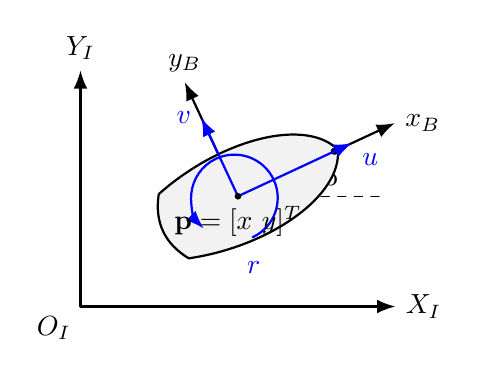
\begin{tikzpicture}[>=Latex, line cap=round, line join=round]
% ---------- parameters ----------
\def\psi{25}         % heading angle (deg)
\def\L{2.4}          % boat length scale
\def\B{1.0}          % boat width scale

% ---------- inertial frame ----------
\coordinate (O) at (0,0);
\draw[->,thick] (O) -- (4,0) node[right] {$X_I$};
\draw[->,thick] (O) -- (0,3) node[above] {$Y_I$};
\node[below left] at (O) {$O_I$};

% ---------- boat pose ----------
\coordinate (C) at (2,1.4); % boat center in inertial frame

% heading reference line + psi
\draw[dashed] (C) -- ++(1.8,0);
\draw[->] (C) ++(0.8,0) arc (0:\psi:0.8);
\node at ($(C)+(1.1,0.25)$) {$\psi$};

% ---------- body frame axes ----------
\begin{scope}[shift={(C)}, rotate=\psi]
  \draw[->,thick] (0,0) -- (2.2,0) node[right] {$x_B$};
  \draw[->,thick] (0,0) -- (0,1.6) node[above] {$y_B$};
  \node[below left] at (0,0) {$O_B$};

  % ---------- simple USV silhouette ----------
  % hull (capsule-like)
  \draw[thick, fill=gray!10]
    (-0.9,0.45) .. controls (0.1,0.75) and (1.2,0.55) .. (1.4,0)
    .. controls (1.2,-0.55) and (0.1,-0.75) .. (-0.9,-0.45)
    .. controls (-1.1,-0.15) and (-1.1,0.15) .. (-0.9,0.45) -- cycle;

  % bow marker
  \fill (1.35,0) circle (1.3pt);

  % ---------- velocities ----------
  \draw[->,blue,thick] (0,0) -- (1.6,0) node[below right] {$u$};
  \draw[->,blue,thick] (0,0) -- (0,1.1) node[left] {$v$};
  \node[blue] at (-0.2,-0.9) {$r$};
  \draw[->,blue,thick] (0,0) ++(-0.05,-0.55) arc (-90:200:0.55);

\end{scope}

% label boat center in inertial frame
\fill (C) circle (1.2pt);
\node[below] at (C) {$\mathbf{p}=[x\ y]^T$};

\end{tikzpicture}
% ======================

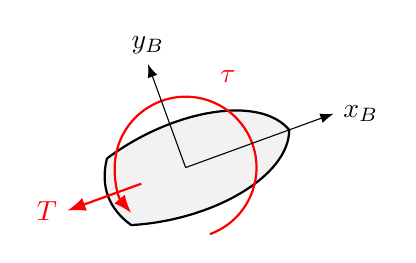
\begin{tikzpicture}[>=Latex]
\begin{scope}[shift={(0,0)}, rotate=20]
  % hull
  \draw[thick, fill=gray!10]
    (-0.9,0.45) .. controls (0.1,0.75) and (1.2,0.55) .. (1.4,0)
    .. controls (1.2,-0.55) and (0.1,-0.75) .. (-0.9,-0.45)
    .. controls (-1.1,-0.15) and (-1.1,0.15) .. (-0.9,0.45) -- cycle;

  % thrust T along body x
  \draw[->,red,thick] (-0.6,0) -- (-1.6,0) node[left] {$T$};

  % yaw moment tau around z
  \draw[->,red,thick] (0,0) ++(0.0,-0.9) arc (-90:200:0.9);
  \node[red] at (0.9,0.9) {$\tau$};

  % body axes (optional)
  \draw[->] (0,0) -- (2.0,0) node[right] {$x_B$};
  \draw[->] (0,0) -- (0,1.4) node[above] {$y_B$};
\end{scope}
\end{tikzpicture}
% =============================
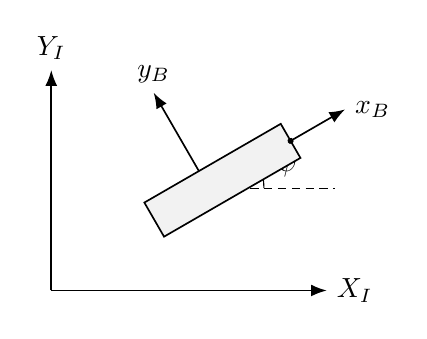
\begin{tikzpicture}[>=Latex]

% styles
\tikzset{
  axis/.style={->, line width=0.6pt},
  body/.style={draw, line width=0.6pt, fill=gray!10},
  ref/.style={densely dashed, line width=0.4pt},
}

% inertial frame
\draw[axis] (0,0) -- (3.5,0) node[right] {$X_I$};
\draw[axis] (0,0) -- (0,2.8) node[above] {$Y_I$};

% USV center
\coordinate (C) at (2.0,1.3);
\fill (C) circle (1pt);

% heading reference
\draw[ref] (C) -- ++(1.6,0);

% heading angle
\draw[->, line width=0.4pt] (C) ++(0.7,0) arc (0:30:0.7);
\node at ($(C)+(1.0,0.3)$) {$\psi$};

% body frame and hull
\begin{scope}[shift={(C)}, rotate=30]
  % body axes
  \draw[axis] (0,0) -- (2.0,0) node[right] {$x_B$};
  \draw[axis] (0,0) -- (0,1.4) node[above] {$y_B$};

  % simplified hull (rigid body)
  \draw[body] (-0.8,-0.25) rectangle (1.2,0.25);

  % bow marker
  \fill (1.2,0) circle (1.1pt);
\end{scope}

\end{tikzpicture}
% ============================
\begin{tikzpicture}[>=Latex]

% ---------- styles ----------
\tikzset{
  axis/.style={->, line width=0.6pt},
  label/.style={font=\small}
}

% ---------- origin ----------
\coordinate (O) at (0,0);
\fill (O) circle (1.2pt);
\node[below left] at (O) {$O_N$};

% ---------- NED axes ----------
% X_N (North / Forward)
\draw[axis] (O) -- (1.8,1.2)
  node[right, label] {$X_N$};

% Y_E (East / Right)
\draw[axis] (O) -- (1.8,-1.2)
  node[right, label] {$Y_E$};

% Z_D (Down)
\draw[axis] (O) -- (0,-2.5)
  node[below, label] {$Z_D$};

\end{tikzpicture}
% =====================
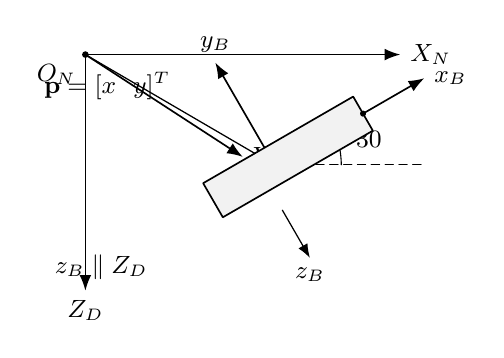
\begin{tikzpicture}[>=Latex, line cap=round, line join=round]

% ---------------- styles ----------------
\tikzset{
  axis/.style={->, line width=0.6pt},
  axisThin/.style={->, line width=0.45pt},
  ref/.style={densely dashed, line width=0.4pt},
  body/.style={draw, line width=0.6pt, fill=gray!10},
  label/.style={font=\small}
}

% ---------------- parameters ----------------
\def\psi{30}              % heading angle (deg)
\coordinate (O) at (0,0); % NED origin
\coordinate (C) at (2.4,-1.4); % USV position in NED (for drawing)

% ---------------- NED inertial frame ----------------
\fill (O) circle (1.2pt);
\node[below left, label] at (O) {$O_N$};

% X_N : forward (North)
\draw[axis] (O) -- (4.0,0) node[right, label] {$X_N$};

% Y_E : right (East)  (drawn slanted to suggest "right" in a pseudo-3D way)
\draw[axis] (O) -- (2.0,-1.3) node[right, label] {$Y_E$};

% Z_D : down
\draw[axis] (O) -- (0,-3.0) node[below, label] {$Z_D$};

% ---------------- position vector ----------------
\fill (C) circle (1.2pt);
\draw[axisThin] (O) -- (C) node[midway, above left, label] {$\mathbf{p}=[x\ \ y]^T$};

% Reference direction at C (parallel to X_N)
\draw[ref] (C) -- ++(1.9,0);

% Heading angle psi (rotation about Z_D)
\draw[->, line width=0.4pt] (C) ++(0.85,0) arc (0:\psi:0.85);
\node[label] at ($(C)+(1.2,0.32)$) {$\psi$};

% ---------------- body frame + simplified USV ----------------
\begin{scope}[shift={(C)}, rotate=\psi]
  % body axes
  \draw[axis] (0,0) -- (2.2,0) node[right, label] {$x_B$};
  \draw[axis] (0,0) -- (0,1.5) node[above, label] {$y_B$};

  % simplified hull (rigid body silhouette)
  \draw[body] (-0.9,-0.25) rectangle (1.3,0.25);
  % bow marker
  \fill (1.3,0) circle (1.1pt);

  % optional: show z_B direction (aligned with Z_D)
  \draw[axisThin] (-0.2,-0.55) -- (-0.2,-1.25) node[below, label] {$z_B$};
\end{scope}

% optional: note alignment (keep subtle)
\node[label] at (0.2,-2.7) {$z_B \parallel Z_D$};

\end{tikzpicture}
% ============================



\end{document}
